\chapter{Estado del arte}
\label{chap:estado_arte}

En este capítulo se presentan los principales conceptos y trabajos previos relacionados con el análisis de la cobertura en redes celulares. Para ello, se explica el modelado de la propagación y de las antenas, las comunicaciones críticas y V2X, la maximización de la cobertura y las herramientas existentes para la simulación del canal en escenarios tridimensionales.

\section{Redes celulares}

Las comunicaciones móviles tienen un papel fundamental en la sociedad actual, ya que permiten mantener la conectividad mientras los usuarios se desplazan. Para ofrecer este servicio en áreas extensas, las redes móviles dividen su área de cobertura en distintas zonas geográficas.

Estas redes se denominan redes celulares y cada una de esas zonas recibe el nombre de celda. Según la Unión Internacional de Telecomunicaciones (ITU), una celda es el área de cobertura radioeléctrica proporcionada por una estación base o por uno de sus subsistemas, como un sector de antena \cite{itur_m1224}.

\par\medskip
\textbf{Nota: No he encontrado una definición directa en ningún lado, solo se puede extraer de glosarios de la ITU. He encontrado dos glosarios, uno en un apartado dentro de la web de la ITU \url{https://www.itu.int/ITU-D/ict/publications/wtdr_99/material/glossary.html} y la recomendación; he usado la segunda porque es la más reciente (la encontré en las referencias del TFG que me disteis de ejemplo).}
\par\medskip

Esta división en celdas permite organizar la cobertura de una zona amplia y reutilizar los recursos radioeléctricos en distintas áreas. De esta forma, los usuarios pueden desplazarse por el territorio manteniendo la conexión con la red y cambiando de celda cuando sea necesario. La cobertura se refiere al alcance de una red móvil celular y puede medirse en términos de cobertura geográfica o de población cubierta \cite{itur_m1224}.

La arquitectura utilizada por las redes celulares ha evolucionado con las distintas generaciones. En el caso de 5G, el sistema está formado por el equipo de usuario (UE), la red de acceso radio de nueva generación (NG-RAN) y el núcleo de red 5G (5GC), como se muestra en la Figura \ref{fig:arquitectura5g} \cite{3gpp_5g_overview}.

\begin{figure}[H]
    \centering
    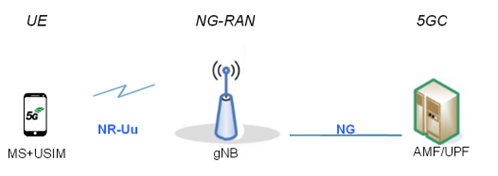
\includegraphics[width=0.8\textwidth, keepaspectratio]{imagenes/estado del arte/5g-fig1.png}
    \caption{Arquitectura general del sistema 5G. Fuente: 3GPP \cite{3gpp_5g_overview}}
    \label{fig:arquitectura5g}
\end{figure}

\par\medskip
\textbf{Nota 1: Como la figura la he cogido de una fuente ¿Se cita así?.}
\par\medskip

\par\medskip
\textbf{Nota 2: Las fuentes están en inglés; cuando se habla de radio coverage, traduzco como cobertura radioeléctrica y radio access dice el chatGPT que se traduce como acceso radio. Me suena un poco raro, pero no se muy bien como traducir eso.}
\par\medskip

Dentro de la NG-RAN, el gNodeB (gNB) actúa como estación base de 5G NR y establece la comunicación radio con el equipo de usuario \cite{3gpp_5g_overview}. Esta comunicación depende de la cobertura proporcionada por la estación base y de las condiciones de propagación de la señal.

El análisis de la cobertura permite determinar las zonas en las que puede establecerse correctamente la comunicación. Para ello, es necesario estudiar la señal recibida en diferentes posiciones y considerar los factores que afectan su propagación.


\section{Modelado}

\subsection{Simulación y modelos}

Para analizar el comportamiento de una red celular antes de su despliegue real, pueden utilizarse simulaciones. Una simulación reproduce la evolución de un sistema real a lo largo del tiempo y permite estudiar su funcionamiento sin realizar experimentos directamente sobre él. Esto resulta útil cuando dichos experimentos son costosos, peligrosos, requieren demasiado tiempo o sus variables de interés son inaccesibles \cite{nist_modeling_simulation}.

Toda simulación requiere un modelo, es decir, una representación simplificada que refleja algunas propiedades del sistema real. Para realizar simulaciones se utilizan principalmente modelos matemáticos, en lugar de modelos físicos u otros medios de representación. Además, las limitaciones y las condiciones de validez del modelo deben tenerse en cuenta al interpretar los resultados \cite{nist_modeling_simulation}.

\par\medskip
\textbf{Nota: Los dos primeros párrafos están sacados de un informe del NIST; supongo que cuenta como fuente de información fiable. El propio NIST cita los libros que utiliza como referencia, pero no los he encontrado online.}
\par\medskip


\subsection{Simulaciones a nivel de enlace y de sistema}

Las simulaciones de comunicaciones inalámbricas pueden realizarse a nivel de enlace o a nivel de sistema:

\begin{itemize}
    \item \textbf{Simulaciones a nivel de enlace:} estudian una comunicación punto a punto entre un transmisor y un receptor. Permiten analizar el comportamiento y las características de un enlace concreto \cite{nvidia_aodt}.

    \item \textbf{Simulaciones a nivel de sistema:} consideran varios enlaces que transmiten y reciben simultáneamente. De esta forma, permiten analizar el comportamiento conjunto de la red y cómo afectan unos enlaces a otros \cite{nvidia_aodt}.
\end{itemize}

Las simulaciones a nivel de enlace se centran, por tanto, en el comportamiento de una comunicación concreta. Por otro lado, las simulaciones a nivel de sistema amplían el análisis a varios transmisores y receptores, permitiendo estudiar su interacción y el rendimiento global del sistema \cite{nvidia_aodt}.


\subsection{Canal de propagación y modelos de canal}

En las comunicaciones inalámbricas, el canal de propagación determina cómo se transmite la señal entre el transmisor y el receptor. Su comportamiento depende de las condiciones del entorno y de la posición de ambos extremos del enlace.

Los modelos de canal se utilizan para representar estas condiciones de propagación mediante distintos escenarios, parámetros y procedimientos, con el objetivo de estimar las características de la señal recibida \cite{etsi138901}.

El 3rd Generation Partnership Project (3GPP) define modelos de canal para distintos escenarios de propagación. Entre ellos se encuentran la microcelda urbana (UMi), la macrocelda urbana (UMa) y los entornos interiores. A su vez, estos modelos distinguen entre condiciones de propagación con línea de visión directa (\textit{Line of Sight}, LOS) y sin línea de visión directa (\textit{Non-Line of Sight}, NLOS) \cite{etsi138901}.


Los escenarios UMi, UMa e interiores se diferencian principalmente por el tipo de entorno, la posición de la estación base y la distancia entre emplazamientos. En UMi, las estaciones base se sitúan por debajo de la altura de los edificios y se consideran entornos como calles, plazas o zonas urbanas abiertas. En UMa, se ubican por encima de los tejados de los edificios circundantes. Por otro lado, los escenarios interiores representan entornos como oficinas y centros comerciales, donde las estaciones base suelen instalarse en paredes o techos a menor altura \cite{etsi138901}.

\par\medskip
\textbf{Nota: Según esta definición, mi escenario sería UMa porque la antena está por encima de los edificios, aunque no llega a los 25 m de altura para UMa según 3GPP. No obstante, como está a decisión del usuario configurar UMi/UMa con ABG y esto es estado del arte, no lo voy a mencionar.}
\par\medskip

Uno de los parámetros principales de estos modelos es la pérdida de propagación, que representa la atenuación experimentada por la señal durante su recorrido. Su cálculo depende del escenario considerado, de la condición LOS o NLOS y de parámetros como la distancia entre el transmisor y el receptor, la frecuencia utilizada y la altura de ambos extremos del enlace \cite{etsi138901}.

Además de la pérdida de propagación, el modelo de 3GPP contempla otros efectos, como el desvanecimiento por sombra, las pérdidas de penetración en edificios y la dispersión temporal y angular de la señal \cite{etsi138901}. La consideración de estos parámetros permite representar con mayor detalle las condiciones de propagación de cada escenario.


\subsection{Modelos de pérdidas de propagación}

\subsubsection{Modelo de pérdidas en el espacio libre}

El modelo de pérdidas en el espacio libre (\textit{Free-Space Path Loss}, FSPL) representa la pérdida de señal producida al propagarse entre un transmisor y un receptor en condiciones de espacio libre. Cuando la distancia entre las antenas es mucho mayor que la longitud de onda, puede calcularse mediante la siguiente expresión \cite{itur_p341}:

\begin{equation}
    L_{\mathrm{bf}}\,(\mathrm{dB})=20\log_{10}\left(\frac{4\pi d}{\lambda}\right)
\end{equation}

donde $d$ es la distancia entre las antenas, expresada en metros, y $\lambda$ es la longitud de onda de la señal, también expresada en metros.

Teniendo en cuenta que $c=\lambda f$, la expresión también puede escribirse como:

\begin{equation}
    L_{\mathrm{bf}}\,(\mathrm{dB})=20\log_{10}\left(\frac{4\pi d f}{c}\right)
\end{equation}

donde $f$ es la frecuencia de la señal, expresada en hercios, y $c$ es la velocidad de propagación de la luz, expresada en metros por segundo.

\par\medskip
\textbf{Nota: Es la de los apuntes de TD, cogí la fuente que estaba puesta en el campus virtual. El resto de fuentes usaba otra versión de L = 32.4 + 20log... que no he usado nunca.}
\par\medskip


\subsubsection{Modelo Alpha-Beta-Gamma}

El modelo Alpha-Beta-Gamma (ABG) es un modelo de pérdidas de propagación a gran escala que expresa las pérdidas en función de la distancia entre el transmisor y el receptor y de la frecuencia de la señal. Este modelo ha sido utilizado en estudios de propagación para redes 5G \cite{abg}. Las pérdidas calculadas mediante el modelo ABG se expresan como:

\begin{equation}
\begin{split}
    PL_{\mathrm{ABG}}\,(\mathrm{dB})={}&10\alpha\log_{10}\left(\frac{d}{1\,\mathrm{m}}\right)
    +\beta \\ &+10\gamma\log_{10}\left(\frac{f}{1\,\mathrm{GHz}}\right)
    +X_{\sigma}^{\mathrm{ABG}}
\end{split}
\end{equation}

donde $d$ es la distancia entre el transmisor y el receptor, expresada en metros; $f$ es la frecuencia de la señal, expresada en GHz; $\alpha$, $\beta$ y $\gamma$ son los coeficientes del modelo; y $X_{\sigma}^{\mathrm{ABG}}$ es una variable aleatoria expresada en dB que representa las variaciones producidas por el desvanecimiento por sombra \cite{abg}.

\par\medskip
\textbf{Nota: Me acabo de dar cuenta (19/07/2026) de que en la fuente (la saqué de  tu TFG, asi que es la misma) pone que esta ecuación solo se cumple cuando d es mayor o igual a 1 m. En el mapa de calor, si ponemos un mapa de 1x1x1 metros con un tamaño de vóxel de 0'1, ninguna medida sería válida porque los 1000 vóxeles del mapa de calor se encuentran a una distancia menor a 1 m.}

\textbf{¿Ignoramos esa condición? No la he añadido a la fórmula por ese mismo motivo. Otra opción es que si se encuentra un receptor a menos de 1m se calculen pérdidas como si estuviese a 1 m (eso lo tenía hecho ya pero con 0.001 m).}

\textbf{En principio, pocas medidas debería haber a esa distancia; solo pasaría en el mapa de calor si el tamaño del vóxel es pequeño y están pegados a la antena.}
\par\medskip

Los parámetros del modelo $\alpha$, $\beta$ y $\gamma$ pueden ajustarse a partir de los datos obtenidos para un escenario determinado \cite{abg}.

\par\medskip
\textbf{Nota: He añadido los modelos FSPL y ABG porque son los modelos de pérdidas que se utilizan posteriormente en el simulador. El CI de interiores me lo he salto porque no está implementado y no se hace nada en interiores.}
\par\medskip


La potencia recibida por los receptores también está condicionada por la forma en que la antena distribuye la energía en el espacio. Por esto, el modelado de su patrón de radiación es otro aspecto fundamental para representar el enlace entre el transmisor y el receptor.


\section{Modelado de antenas}

Las características de una antena determinan cómo se distribuye la energía radiada en el espacio. Esta distribución se representa mediante el patrón de radiación, que muestra cómo varía la ganancia de la antena según la dirección de propagación. Para analizar su comportamiento de forma completa, es necesario disponer de un patrón tridimensional que permita conocer la ganancia alrededor de toda la antena.

Sin embargo, la información proporcionada por los fabricantes se limita a los cortes horizontal y vertical. Estos patrones bidimensionales muestran el comportamiento de la antena en dos planos, pero no permiten conocer directamente los valores correspondientes a las direcciones situadas fuera de ellos. Por este motivo, se han desarrollado diferentes métodos para estimar el patrón tridimensional completo a partir de ambos cortes.

Uno de los procedimientos más sencillos y directos consiste en sumar los valores de los patrones horizontal y vertical expresados en escala logarítmica, normalmente en decibelios, para obtener la ganancia correspondiente a cada dirección. Este método es fácil de implementar y puede proporcionar buenos resultados en antenas omnidireccionales con patrones regulares o simétricos. Sin embargo, en antenas directivas o con patrones más complejos, puede dar lugar a errores importantes, especialmente fuera del lóbulo principal \cite{7268850}.

Gil et al. propusieron un método de interpolación para reconstruir el patrón tridimensional de antenas de estación base a partir de los cortes horizontal y vertical. Su procedimiento combina ambos patrones teniendo en cuenta la dirección que se desea estimar \cite{gil2001}.

Este método utiliza toda la información disponible en los cortes horizontal y vertical, por lo que puede conservar las diferencias existentes entre las distintas partes del patrón vertical. No obstante, no puede reconstruir de forma exacta las características del patrón que no aparecen representadas en dichos cortes. Por este motivo, pueden producirse errores en zonas como los lóbulos secundarios o las direcciones alejadas de los planos principales.

Posteriormente, Vasiliadis et al. presentaron un método de aproximación basado en la combinación ponderada de los dos cortes principales. En lugar de sumar directamente ambos valores, el método asigna un peso diferente a cada corte en función de la distancia angular existente entre la dirección que se desea estimar y los planos horizontal y vertical. De este modo, las direcciones reciben una mayor influencia del plano más cercano \cite{vasiliadis2005}.

Esta combinación ponderada permite reducir el error respecto al método de suma directa. Además, el método presenta buenos resultados tanto para antenas omnidireccionales como para antenas directivas. Sin embargo, su funcionamiento depende de un parámetro k, que controla la forma en que se distribuyen los pesos de los cortes horizontal y vertical. Los autores explican que un valor $k = 2$ minimiza el error de la reconstrucción, aunque también indican que el valor más adecuado puede depender de la directividad y de las características de cada antena \cite{vasiliadis2005}.

Otra limitación del método de Vasiliadis se encuentra en la interpretación del corte vertical. El procedimiento utiliza 360 muestras del patrón horizontal y 180 muestras del patrón vertical \cite{vasiliadis2005}. Si las dos mitades del patrón vertical son simétricas, una de ellas puede utilizarse para representar la otra sin que se produzcan diferencias. Sin embargo, cuando el patrón no es simétrico, la reducción del corte vertical implica la pérdida de la información correspondiente a una de sus mitades.

Además de estos métodos, también es posible reconstruir patrones tridimensionales mediante técnicas de \textit{deep learning}. MathWorks proporciona una implementación que utiliza una red neuronal entrenada para estimar un patrón tridimensional a partir de cortes bidimensionales \cite{mathworks_patternfromai}. La red aprende la relación entre los cortes principales y los patrones tridimensionales reconstruidos a partir de un conjunto de antenas utilizadas durante el entrenamiento.

Este método es más difícil de implementar, ya que requiere una gran cantidad de muestras para entrenar y validar el modelo. Sin embargo, el \textit{deep learning} permite reconstruir patrones más complejos que los métodos anteriores.

El modelado del patrón de radiación permite estimar con mayor precisión la ganancia de la antena en cada dirección y, por tanto, analizar cómo se distribuye la cobertura en el escenario. Este análisis resulta especialmente importante en servicios donde la comunicación debe mantenerse incluso en situaciones de emergencia o en condiciones desfavorables.


\section{Comunicaciones críticas}

Las comunicaciones críticas son aquellas utilizadas por organismos de protección pública y atención ante desastres en situaciones donde la vida humana, los bienes u otros valores de la sociedad están en riesgo, especialmente cuando el tiempo es un factor determinante. Estas comunicaciones deben ser seguras, fiables y estar disponibles cuando se necesiten \cite{itur_m2377}.

Debido a la importancia de estas situaciones, las comunicaciones críticas presentan requisitos más exigentes que otros servicios convencionales. Deben ofrecer baja latencia, alta disponibilidad y fiabilidad, capacidad para gestionar un gran número de usuarios y dispositivos, seguridad y mecanismos de prioridad \cite{etsi122280}.

Además, estos sistemas deben permitir el intercambio de distintos tipos de información. 3GPP utiliza el término MCX para agrupar las aplicaciones críticas, entre las que se incluyen \textit{Mission Critical Push To Talk} (MCPTT), para las comunicaciones de voz; \textit{Mission Critical Video} (MCVideo), para la transmisión de vídeo en tiempo real; y \textit{Mission Critical Data} (MCData), para el intercambio de datos en tiempo real \cite{etsi122280}.

Estos servicios pueden utilizarse en aplicaciones de seguridad pública y en otros ámbitos que requieren una comunicación fiable, como las operaciones marítimas y determinados sectores comerciales \cite{etsi122280}. También permiten realizar comunicaciones entre usuarios individuales y grupos, facilitando el intercambio de información entre los distintos participantes de una operación.

En este contexto, la cobertura es un aspecto especialmente importante. La pérdida de conexión o una calidad insuficiente de la señal puede impedir el intercambio de voz, vídeo o datos en situaciones donde la comunicación resulta necesaria. Por este motivo, el análisis de la propagación permite identificar zonas con problemas de cobertura y estudiar cómo influyen factores como la posición de la antena, el patrón de radiación, la distancia y los obstáculos presentes en el entorno.

Las herramientas de simulación permiten realizar este análisis antes de desplegar o modificar una red. Mediante ellas es posible representar la distribución de la señal en un escenario, evaluar la cobertura en distintas posiciones y localizar las zonas en las que las condiciones de comunicación pueden resultar insuficientes para este tipo de comunicaciones.


\section{V2X y comunicaciones vehiculares}

Las comunicaciones vehiculares permiten intercambiar información entre los vehículos y otros elementos de su entorno. Estas se agrupan bajo el termino V2X, procente de \textit{Vehicle-to-Everything}, y permiten que vehículos, infraestructuras, servidores de aplicaciones y peatones recopilen y compartan información de su entorno para ofrecer servicios relacionados con la seguridad, la eficiencia del tráfico y otras aplicaciones de los sistemas de transporte inteligente \cite{etsi122185}.

3GPP define cuatro tipos de comunicaciones V2X: vehículo a vehículo (\textit{Vehicle-to-Vehicle}, V2V), vehículo a infraestructura (\textit{Vehicle-to-Infrastructure}, V2I), vehículo a red (\textit{Vehicle-to-Network}, V2N) y vehículo a peatón (\textit{Vehicle-to-Pedestrian}, V2P) \cite{etsi122185}.

En las comunicaciones V2V, los vehículos cercanos entre sí intercambian información, como su posición o su movimiento. En V2I, el vehículo se comunica con elementos de la infraestructura, como una unidad situada junto a la carretera, llamada \textit{Roadside Unit} (RSU). En V2N, el vehículo intercambia información con un servidor de aplicaciones a través de la red. Por último, V2P permite la comunicación entre vehículos y usuarios vulnerables, como peatones, mediante los dispositivos asociados a cada uno de ellos \cite{etsi122185}.

El intercambio de esta información permite que los vehículos y el resto de elementos conozcan mejor lo que ocurre en su entorno. A partir de estos datos, se pueden desarrollar aplicaciones como los avisos de colisión, la coordinación entre vehículos o la conducción automatizada. Estas aplicaciones pueden contribuir tanto a mejorar la seguridad vial como a aumentar la eficiencia del tráfico \cite{etsi122185}.

Las comunicaciones V2X tienen requisitos específicos debido al movimiento de los vehículos y a la necesidad de transmitir información en un tiempo reducido. 3GPP establece requisitos relacionados con la latencia, la fiabilidad, el alcance de la comunicación, la densidad de UE y la velocidad de los vehículos. Por ejemplo, para transferir mensajes entre dos UE que soporten aplicaciones V2V o V2P, se establece una latencia máxima de 100 ms, mientras que, en casos como la detección previa a una colisión, la latencia máxima no puede superar los 20 ms \cite{etsi122185}.

Las aplicaciones V2X más avanzadas se pueden agrupar en cuatro categorías: la formación de grupos de vehículos que circulan de manera coordinada, la conducción avanzada, el intercambio de información procedente de sensores y la conducción remota \cite{etsi122186}. Estos casos pueden requerir el envío frecuente de datos y altos niveles de fiabilidad, especialmente cuando la información recibida se utiliza para tomar decisiones sobre el movimiento del vehículo.

En este tipo de comunicaciones, la cobertura y la calidad de la señal son factores fundamentales. El movimiento de los vehículos modifica continuamente la distancia y la dirección respecto a la antena, mientras que los edificios y otros obstáculos pueden introducir pérdidas adicionales. Por ello, el análisis de la propagación permite estudiar cómo varían la potencia recibida y la SNR durante un recorrido e identificar zonas en las que la comunicación vehicular puede no ser viable.


\section{Maximización de la cobertura}

Como se ha explicado anteriormente en este capítulo, cada celda representa el área de cobertura proporcionada por una estación base. La maximización de la cobertura busca ampliar las zonas de la celda en las que los UE pueden acceder a la red y mantener correctamente la comunicación, reduciendo los puntos donde la cobertura es insuficiente.

La maximización de la cobertura no implica simplemente aumentar el alcance de la celda. También es necesario evitar que la señal se extienda más allá de la zona prevista, ya que esto puede aumentar el solapamiento con otras celdas y generar más interferencias. Por este motivo, es necesario mantener un equilibrio entre cobertura y capacidad \cite{etsi132522}.

Para mejorar la cobertura, se pueden optimizar parámetros como la potencia de transmisión, la inclinación de la antena y su orientación horizontal \cite{etsi132522}. Estos parámetros modifican la celda, ya que afectan a la potencia recibida y a las direcciones en las que se concentra la radiación.

El aumento de la potencia de transmisión eleva la potencia recibida por los UE y puede ampliar la zona de la celda en la que la señal supera el nivel necesario para mantener la comunicación. Sin embargo, su valor debe ajustarse para evitar que la cobertura alcance zonas más alejadas de lo previsto.

La inclinación y la orientación horizontal de la antena permiten dirigir el lóbulo principal hacia las zonas donde se desea proporcionar una mayor cobertura. La forma del patrón de radiación determina la ganancia disponible en cada dirección y, por tanto, la distribución espacial de la cobertura.

Uno de los problemas que se busca reducir son los huecos de cobertura. 3GPP define un hueco de cobertura como una zona donde la intensidad de la señal queda por debajo del umbral necesario para que un UE acceda a la red o donde la SINR de la celda servidora y de las celdas vecinas no permite mantener el servicio básico. Estos huecos pueden deberse a obstáculos físicos, a una configuración inadecuada de los parámetros de la antena o a una planificación radioeléctrica insuficiente \cite{etsi132522}.

También pueden aparecer zonas de cobertura débil, en las que la intensidad de la señal, la SNR o la SINR quedan por debajo del nivel necesario para alcanzar el rendimiento previsto. A su vez, puede producirse una cobertura excesiva cuando la señal de una celda alcanza zonas mucho más alejadas de las planificadas \cite{etsi132522}.

Por tanto, la maximización de la cobertura requiere estudiar la distribución de la señal dentro de la celda y ajustar los parámetros de la antena en función del entorno. Las herramientas de simulación permiten comparar distintas configuraciones de potencia, orientación y patrón de radiación, así como localizar huecos y zonas de cobertura débil antes de realizar cambios en una red real.


\section{Herramientas de simulación de canal tridimensional}

El análisis de la cobertura en escenarios tridimensionales puede realizarse mediante herramientas que combinan la representación del entorno con modelos de propagación. Estas plataformas permiten establecer transmisores y receptores dentro de un escenario digital, configurar sus parámetros y estudiar cómo afectan la geometría y los materiales del escenario a la propagación de la señal.

\par\medskip
\textbf{Nota: Me dijiste (José Javier) que debía meter este apartado en el estado del arte y mover el de soluciones alternativas al estado del arte. No obstante, al hacerlo, veo que son equivalentes; he quitado el de soluciones alternativas y lo he metido todo aquí. No sé si el de soluciones alternativas se refería a otra cosa.}
\par\medskip

\subsection{NVIDIA Aerial Omniverse Digital Twin}

NVIDIA Aerial Omniverse Digital Twin (AODT) es una plataforma de gemelo digital para la investigación y el desarrollo de redes 6G. Esta herramienta utiliza NVIDIA Omniverse para representar el entorno tridimensional y tecnologías de \textit{ray tracing} mediante GPU para simular el comportamiento de la propagación radioeléctrica \cite{nvidia_aodt}.

AODT permite realizar simulaciones a nivel de sistema, considerando varios transmisores y receptores que funcionan simultáneamente. La plataforma puede utilizarse tanto en escenarios formados por una única estación base y un bajo número de UE, como en representaciones urbanas con cientos de estaciones base y miles de UE \cite{nvidia_aodt}.

Para modelar la propagación, AODT utiliza un solucionador electromagnético basado en \textit{ray tracing}. Este modelo tiene en cuenta reflexiones, difracciones y efectos de dispersión difusa direccional. También permite definir los patrones de radiación de los elementos de antena, por lo que la ganancia depende de la dirección de propagación \cite{nvidia_aodt}.

AODT combina la simulación del entorno radioeléctrico con simuladores de la red de acceso radio y de los UE. De esta forma, permite estudiar tanto la propagación como el rendimiento a nivel de sistema y probar distintos algoritmos antes de desplegarlos en una red real \cite{nvidia_aodt}.

En la Figura \ref{fig:aodt} se muestra un escenario urbano representado mediante AODT, junto con las trayectorias de propagación simuladas entre el transmisor y el receptor.

\begin{figure}[H]
    \centering
    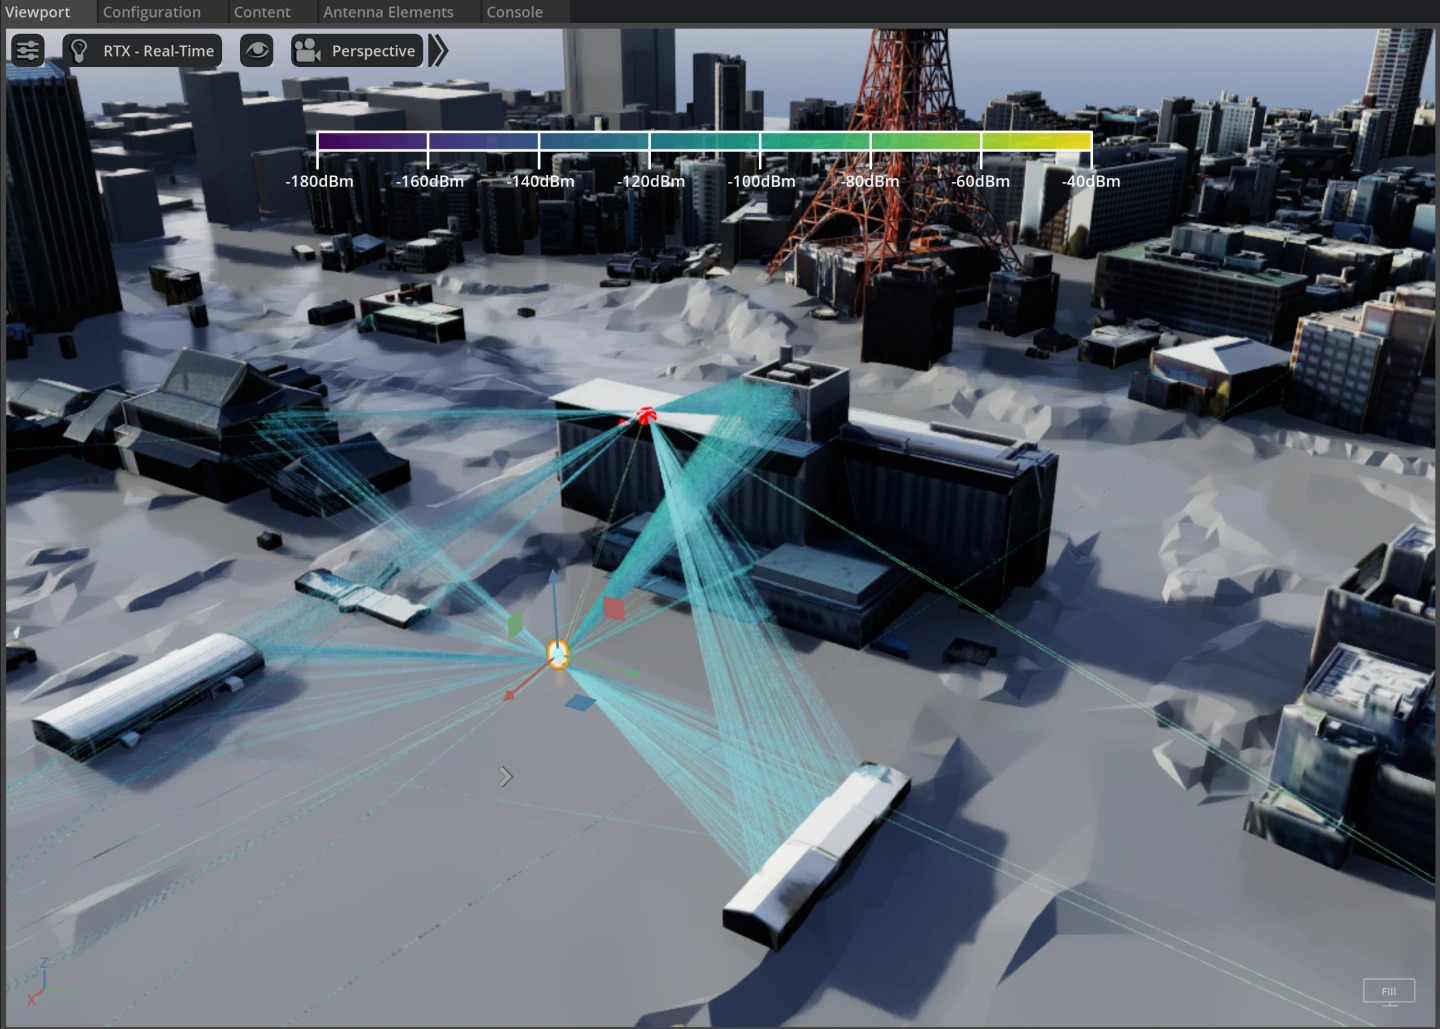
\includegraphics[width=0.9\textwidth]{imagenes/estado del arte/nvidia_aodt.jpg}
    \caption{Simulación de la propagación radioeléctrica mediante NVIDIA AODT. Fuente: NVIDIA \cite{nvidia_aodt}}
    \label{fig:aodt}
\end{figure}


\subsection{Sionna RT}

Sionna RT es una biblioteca de código abierto desarrollada por NVIDIA para el modelado de la propagación radioeléctrica mediante \textit{ray tracing}. Permite representar escenarios tridimensionales y calcular el comportamiento del canal entre transmisores y receptores situados en diferentes posiciones \cite{sionna_rt}.

La herramienta está construida sobre Mitsuba 3, un sistema de renderizado orientado a la simulación del transporte de la luz y al renderizado diferenciable. En Sionna RT, Mitsuba 3 se utiliza para cargar, representar y gestionar la geometría y los materiales de los escenarios tridimensionales \cite{sionna_rt}.

Los escenarios pueden crearse, editarse y exportarse mediante Blender utilizando el complemento Mitsuba-Blender. También es posible generar escenarios a partir de datos de OpenStreetMap mediante complementos específicos de Blender \cite{sionna_rt}.

Una vez cargado el escenario, Sionna RT permite definir transmisores, receptores, patrones de antena y propiedades radioeléctricas de los materiales. A partir de estos elementos, puede calcular los caminos de propagación y obtener parámetros como los coeficientes del canal, los retardos o los ángulos de llegada y salida \cite{sionna_rt}.

En la Figura \ref{fig:sionna_rt} se muestra un escenario urbano de Múnich representado mediante Sionna RT, junto con las trayectorias de propagación calculadas entre un transmisor y un receptor.

\begin{figure}[H]
    \centering
    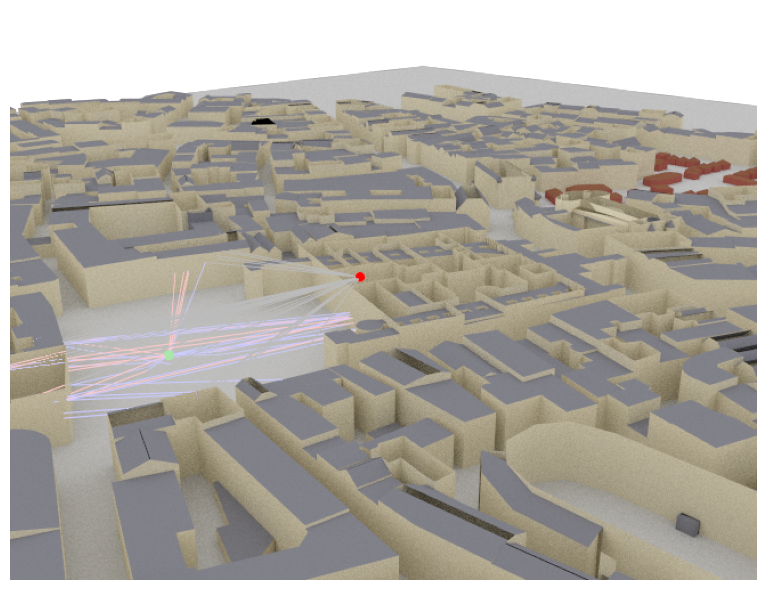
\includegraphics[width=0.9\textwidth]{imagenes/estado del arte/rt_tutorials_Introduction_33_0.png}
    \caption{Escenario urbano y trayectorias de propagación calculadas en Sionna RT. Fuente: NVIDIA \cite{sionna_rt}}
    \label{fig:sionna_rt}
\end{figure}

\subsection{Altair WinProp}

Altair WinProp es una herramienta orientada al análisis de la propagación radioeléctrica y a la planificación de redes inalámbricas. Permite estudiar la cobertura en distintos tipos de escenarios, como entornos urbanos, rurales, industriales e interiores, y dispone de modelos de propagación y funciones de planificación para diferentes tecnologías de comunicación \cite{altair_winprop}.


\subsection{MATLAB}

MATLAB también tiene herramientas para analizar y visualizar la propagación radioeléctrica en escenarios tridimensionales. Mediante \textit{Site Viewer} es posible colocar transmisores y receptores, representar enlaces y generar mapas de cobertura y de SINR tanto en entornos exteriores como interiores \cite{mathworks_rfpropagation}.

Además, MATLAB permite utilizar modelos de \textit{ray tracing} para calcular los caminos seguidos por la señal y estudiar cómo influyen la geometría y los materiales del escenario en la propagación.

En la Figura \ref{fig:matlab_sinr} se muestra un mapa de SINR generado sobre un escenario geográfico. La escala de colores permite identificar las zonas con mejores y peores condiciones de recepción.

\begin{figure}[H]
    \centering
    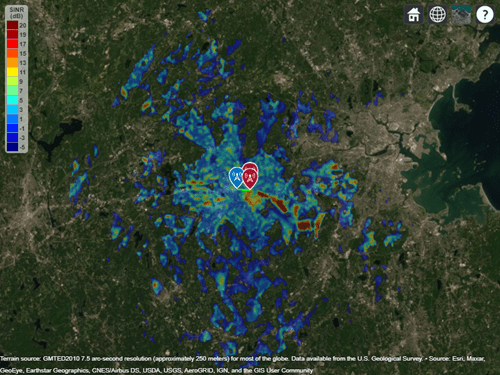
\includegraphics[width=0.8\textwidth]{imagenes/estado del arte/RFPropagationAndVisualizationExample_05.png}
    \caption{Representación de la distribución de la SINR sobre un escenario geográfico mediante MATLAB. Fuente: MathWorks \cite{mathworks_rfpropagation}}
    \label{fig:matlab_sinr}
\end{figure}